%\newpage
\subsection{Implementation of Android client example applications}

The prototype of client-server application was designed during this research project.
The application program was executed on the Google Android operating system powered hardware.


Main idea of this application is the remote wireless control of some electronic device. 
The controlled device example here is a coffee machine, that has some functions like preparing a cup of coffee.
We needed that these functions became available for remote control.

The developed application is a small application with trivial user interface, which allows to prepare products by selecting a product from a small catalogue. 
The screen shot of a ready application is provided  in the \autoref{fig:android_app_screen}

\begin{center}
 \begin{figure}[h]
	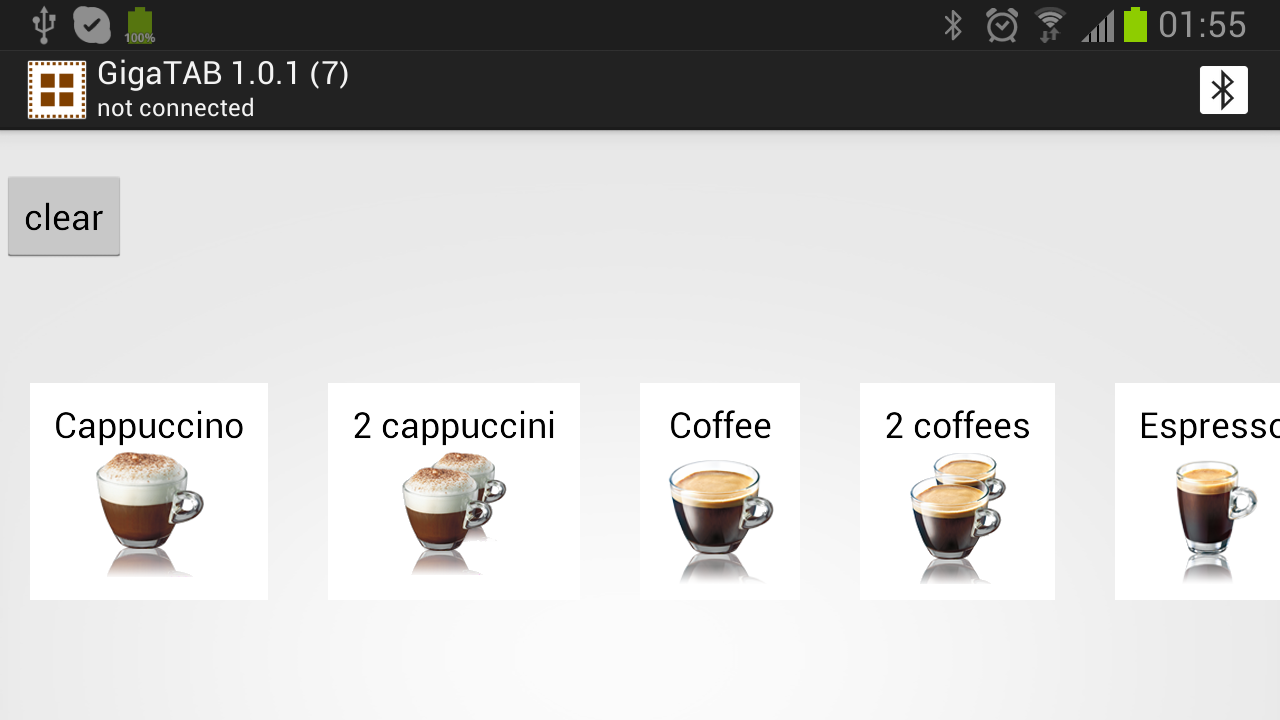
\includegraphics[width=\textwidth]{../images/implementation/android_app_screen.png}
	\caption{The Android application visual interface }
	\label{fig:android_app_screen}
 \end{figure}
\end{center}

The usage scenario starts from the connection to coffee machine.
There is a small button with Bluetooth icon in the top right corner of the application.
This button activates a device select dialog, where you can find a remote device by name and MAC address and connect by selecting it in the list.
When connection is established some available products become showed in the horizontal list layout.
It is able to point to each of these products and open a dialog box with detailed information about each product.
User can start coffee preparing from that dialog.
While operation is in progress, it is still possible to cancel the product preparing operation.

I will not cover in details the whole process of the user interface and application creation.
This is out of the scope of this research work and it requires some additional domain knowledge. 
You need to get familiar with Google Android development tools,
read a documentation course, follow the tutorials and study by doing.
There are available lots of application examples and it is not very hard to produce a similar application.
This application is partially based on the Bluetooth chat communication example from the Android Software development kit.

Whole communication is performed over wireless Bluetooth protocol.
It is assumed, that Bluetooth is the abstract transport that can send data bytes over radio link.
The Android Bluetooth API functions can search to nearby Bluetooth devices and provide you a list of \texttt{BluetoothDevice} objects.
You can find your wireless device in that list and tell the Android OS to connect to that device. 
This device list is also used to fill a device choosing graphical dialog described before.

When devices get connected  it is able to receive a communication socket object and get a standard \texttt{java.io.InputStream} and \texttt{java.io.OutputStream} from that.
This is a final step of establishing the communication and it is able to transfer data over received stream objects.


The client RPC library is connected to these streams and it is able to communicate with a remote device over the wireless serial interface.
RPC calls may be started right after application gets connected to the Bluetooth input and output streams.


Now it is up to your imagination how to use and extend this remote embedded service.
You can implement any rich functionality and create whatever complex system you want or your hardware resources allow you.
This extensible service oriented embedded architecture allows you to do so.
